\chapter{Resultados}
\label{chap:result}
O principal objetivo deste projeto foi adaptar o site do portfólio às expectativas e
 necessidades da Jhenifer. Durante essa jornada, conseguimos avançar de forma
 consistente, completando todas as etapas previstas para o GATE A. Isso incluiu um
 levantamento detalhado dos requisitos junto à cliente, definição da estrutura
 organizacional, criação do cronograma preliminar e realização de reuniões e workshops
 essenciais para garantir que tudo estivesse bem alinhado.
 No GATE B, continuamos evoluindo e validando as principais peças de modelagem do
 sistema, como o diagrama de sequência e o diagrama de classes. Além disso, realizamos
 um comitê com a cliente, o que foi fundamental para validar parte das entregas e garantir
 que o projeto estivesse indo na direção certa.
 Em resumo, tudo o que foi feito até agora resultou em um planejamento bem estruturado,
 na criação das modelagens necessárias para aprimorar o site e na validação inicial junto à
 cliente. Com isso, estabelecemos uma base sólida para dar continuidade ao projeto e
 concluí-lo conforme os objetivos planejados.
% %--------- NEW SECTION ----------------------
% \section{Testes unitários}
% \label{sec:testu}
% \lipsum[1]

% \section{Integração do sistema}
% \label{sec:intsis}
% \lipsum[1]

% %--------- NEW SECTION ----------------------
% \section{Testes integrados}
% \label{sec:testi}
% \lipsum[1]

\section{Diagrama de classes}
\label{sec:class}
O diagrama de classes é uma representação visual das classes do sistema e seus relacionamentos. Ele é utilizado para descrever a estrutura do sistema e como as classes interagem entre si. A Figura \ref{fig:Diagrama_de_classes} apresenta o diagrama de classes do sistema desenvolvido.
\begin{figure} [h!]	
    \centering
    \caption{Meu diagrama de classes}
    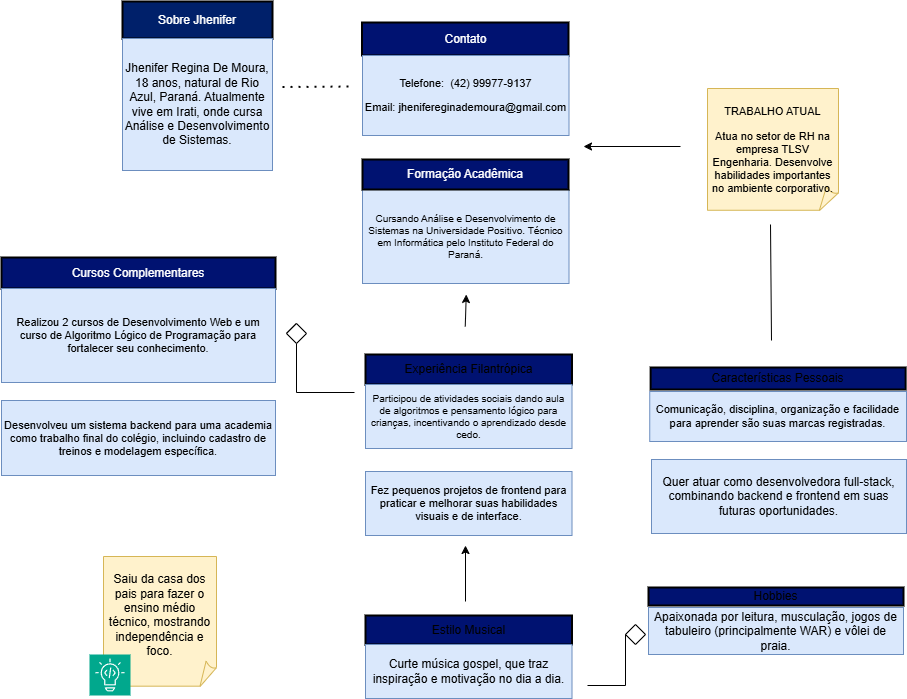
\includegraphics[width=0.8\textwidth]{Figures/Diagrama_de_Classes.png}
    \caption*{Fonte: Autoria própria.}
    \label{fig:Diagrama_de_classes}
\end{figure}

favor olhar a seção \ref{sec:class}.


\section{Diagrama de casos de uso}
\label{sec:casos}
O diagrama de casos de uso é uma representação visual dos casos de uso do sistema e os atores envolvidos. Ele é utilizado para descrever as funcionalidades do sistema e como os usuários interagem com ele. A Figura \ref{fig:casos_de_uso} apresenta o diagrama de casos de uso do sistema desenvolvido.
\begin{figure} [h!] 
    \centering
    \caption{Meu diagrama de casos de uso}
    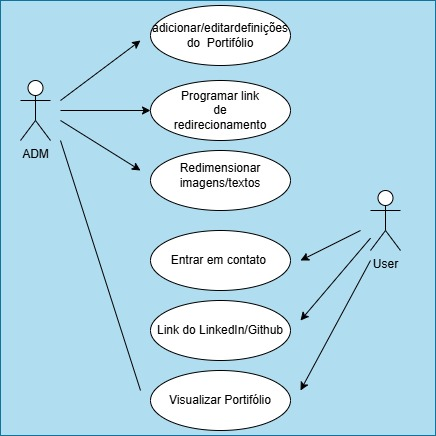
\includegraphics[width=0.8\textwidth]{Figures/casos_de_uso.jpg}
    \caption*{Fonte: Autoria própria.}
    \label{fig:casos_de_uso}
\end{figure}

favor olhar a seção \ref{sec:casos}.

\section{Diagrama de sequência}
\label{sec:sequencia}   
O diagrama de sequência é uma representação visual da interação entre os objetos do sistema ao longo do tempo. Ele é utilizado para descrever como os objetos interagem entre si para realizar uma determinada funcionalidade. A Figura \ref{fig:Diagrama_de_sequencia} apresenta o diagrama de sequência do sistema desenvolvido. 
\begin{figure} [h!] 
    \centering
    \caption{Meu diagrama de sequência}
    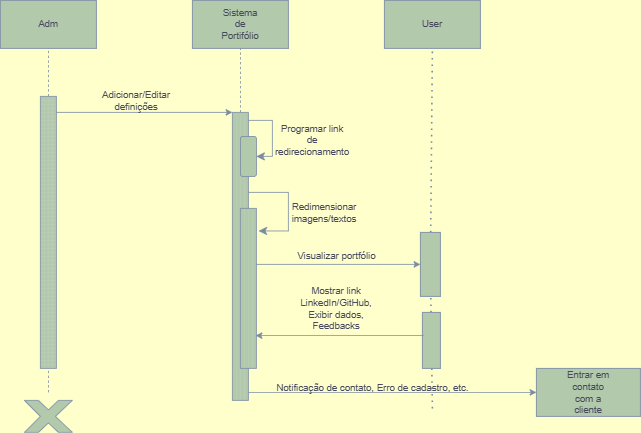
\includegraphics[width=0.8\textwidth]{Figures/Diagrama_de_sequencia.png}
    \caption*{Fonte: Autoria própria.}
    \label{fig:Diagrama_de_sequencia}
\end{figure}

favor olhar a seção \ref{sec:sequencia}.



